\section{Castlevania: Aria of Sorrow}

\begin{figure}[htbp]
\begin{center}
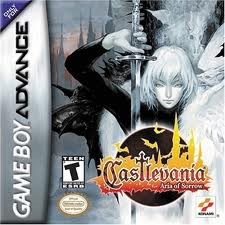
\includegraphics[width=.60\textwidth]{./imagenes/castlevaniaAOS.jpg}
\caption{Castlevania: Aria of Sorrow}
\label{Zelda: Skyward Sword}
\end{center}
\end{figure}
Castlevania\footnote{Iván Aveiga}: Aria of Sorrow \footnote{\url{http://es.games.konami-europe.com/game.do?idGame=31}} es un juego desarrollado por Konami para la plataforma de Game Boy Advance (GBA). Es el año 2035 y Soma Cruz tiene que enfrentarse a Drácula, debe enfrentarse a enemigos para poder evitar que el Caos se una con el mundo y destruya la humanidad. Soma debe luchar contra Graham Jones que cree que es la resurrección Drácula, pero al final Soma debe luchar contra si mismo para evitar transformarse en Drácula.

Soma tiene el poder de adquirir las habilidades de los enemigos que destruye, capturando su alma. Esto le permite enfrentarse a distintos enemigos y ganar con facilidad

\subsubsection{¿Por qué es uno de mis juegos favoritos?}
\begin{itemize}
	\item Fue el primer juego de Castlevania que lo jugué completamente.
	\item La trama del juego es muy elaborada, con dos finales.
	\item La captura de almas para usarlas como habilidad fue implementada por primera vez.
	\item Los enemigos son en su mayoría pertenecientes a distintas mitologías, tenemos enemigos como:
		\begin{itemize}
			\item Poseidón.
			\item Mandrágora.
			\item Medusa.
			\item Sucubus.
			\item Incubus.
			\item Caos
		\end{itemize}	
\end{itemize}